%!TEX root = ../../main.tex

\chapter{Item collections}
\index{Item collection}


\section{Empty content indicator}
\label{sec:empty_content_indicator}

\index{Layout content!Empty content}
\index{Item collection!Empty content}

If one should have that the content is a dynamic collection of items and that collection is empty one should indicate that there are no items avaiable. This indicator should be a gray text \todo{refer to gray} like seen in \figref{fig:empty_content_noitems}.

\begin{figure}
    \centering
    \begin{subfigure}[t]{0.4\textwidth}
        \centering
        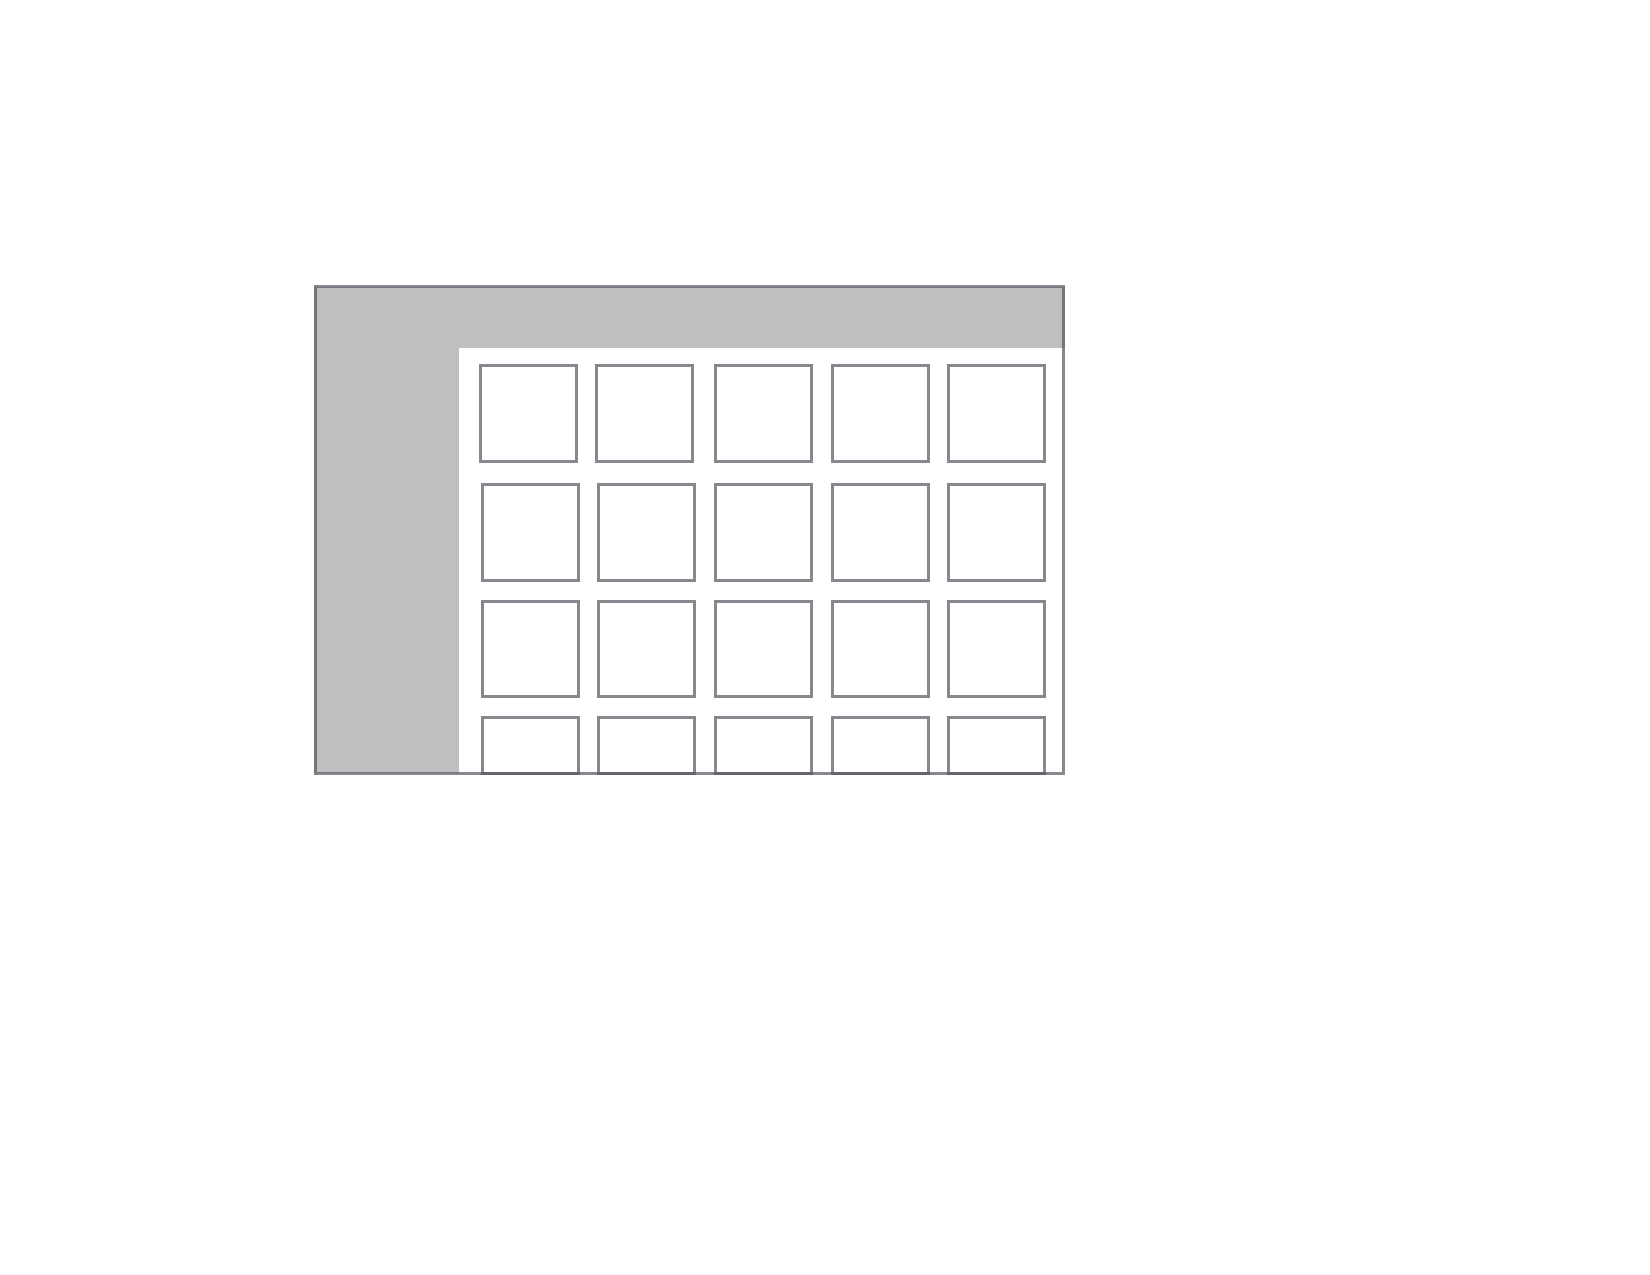
\includegraphics[scale=0.4]{item_collection_items}
        \caption{Content with items}
        \label{fig:empty_content_items}
    \end{subfigure}
    \hspace{5em} 
    \begin{subfigure}[t]{0.4\textwidth}
        \centering
        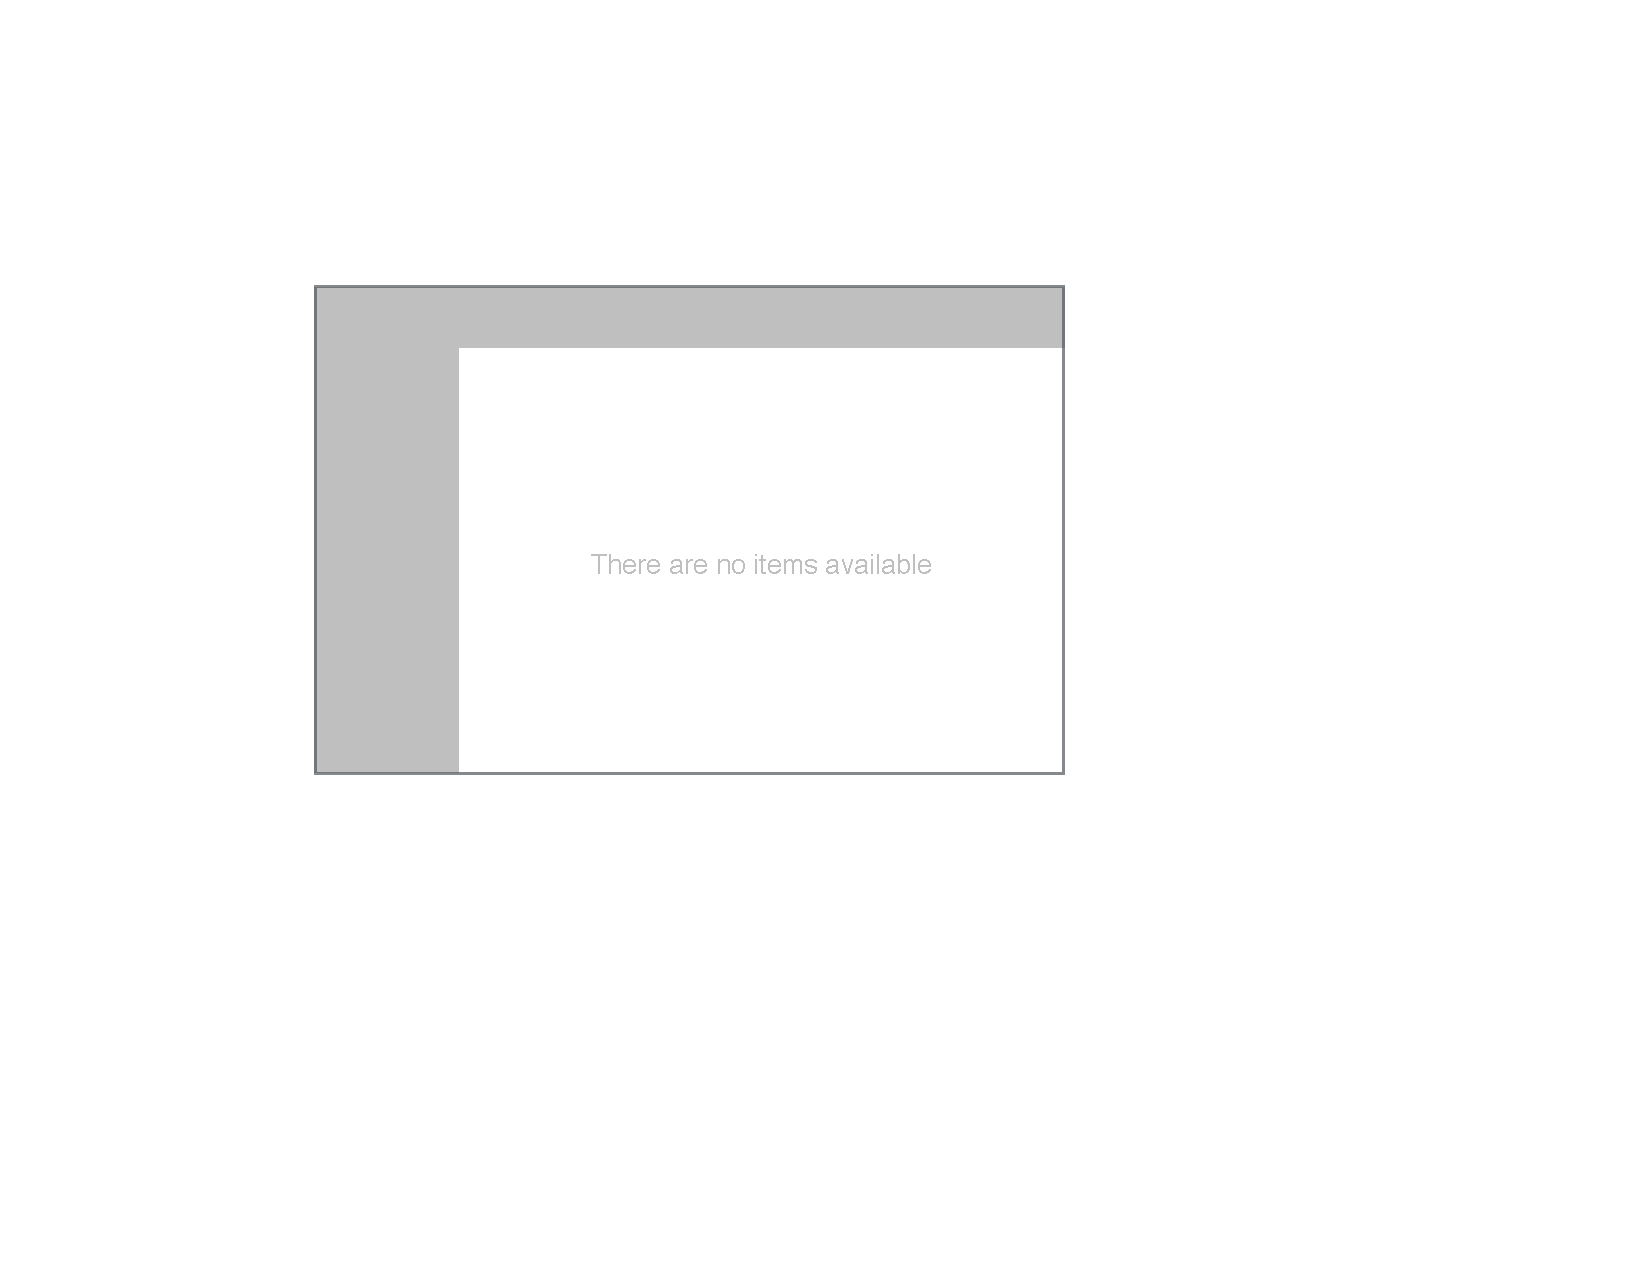
\includegraphics[scale=0.4]{item_collection_noitems}
        \caption{Content with no items}
        \label{fig:empty_content_noitems}
    \end{subfigure}
    
    \caption{Empty content indicator}
    \label{fig:empty_content}
\end{figure}